\chapter{Theory}
\section{Functionality of a Current Transformer}
A current transformer (CT) is an instrument transformer that creates an AC-signal on its secondary side that is proportional to the alternating current on its primary side. This is especially suitable if the current on the primary side is too high to measure because the CT provides a current on the secondary side that can be measured. A current transformer is suitable for current waveshapes and amplitudes from microamperes to megaamperes in high voltage circuits. Another advantage over a shunt resistance is due to the galvanic isolation of the secondary side from the primary. This galvanic isolation prohibits large currents on the secondary side during a  which might destroy the Butterworth-Filter or the Digital-to-Analog-Converter (DAC). 


\section{Debye model}
The polarization effects in a dielectric material can be characterized by the relative permittivity and the dielectric loss factor. 
For linear materials the polarization can be described by a network model. The Debye-ansatz assumes that the rate of change $ dP_i/dt$ is of the remaining difference between the polarization $P_i(t)$ and the polarization at infinity $P_i(\infty$) is proportional. This results in an exponential decay of the polarization function that towards $P_i(\infty)$. This exponential decay can be modeled with a time constant of a resistor and a capacitor in series ($\tau=R_i \cdot C_i$). 

\subsection{Derivation of maximum tan($\delta$)}
The aim of this section is to derive the formula for the maximum tan($\delta$) of the Debye model in order to adjust its value to a disired one.
\begin{equation}
\epsilon_{eff}^* (\omega) = \frac{C^*(\omega)}{C_0}
\end{equation}

\begin{equation}
\epsilon^* = \epsilon_r-j \cdot \epsilon_r''
\end{equation}


\begin{equation}
\epsilon'_r = \epsilon_{\infty} + \frac{\epsilon_{stat}-\epsilon_{\infty}}{1+(\omega \cdot \tau )^2}
\end{equation}

\begin{equation}
\epsilon''_r = \omega \cdot \tau \cdot \frac{\epsilon_{stat}-\epsilon_{\infty}}{1+(\omega \cdot \tau )^2}
\end{equation}

The loss tangents are given by:
\begin{equation}
tan (\delta) = \frac{\kappa + \omega \cdot \epsilon_0 \cdot \epsilon _r ''}{\omega \cdot \epsilon_0 \cdot \epsilon _r '}
\end{equation}

\begin{equation}
tan (\delta_{L}) = \frac{\kappa}{\omega \cdot \epsilon_0 \cdot \epsilon_r'} \newline
\end{equation}

\begin{equation}
tan (\delta_{pol}) = \frac {\epsilon_r'' } {\epsilon_r'}
\end{equation}


We are measuring in the frequency domain from $10^{-6}$ Hz to $10^{11}$ Hz 

\begin{equation}
\epsilon^*(\omega) = \frac{1}{j \omega  Z^*(\omega) C_0}
\end{equation}

\begin{equation}
Z_0(\omega)=[\frac{1}{R_\infty}+\frac{1}{R_i+\frac{1}{j \omega C_i}}+j \omega C_0]^{-1} = [\frac{1}{R_\infty}+\frac{j \omega C_i}{j\omega R_i  C_i+1}+j \omega C_0]^{-1}
\end{equation}

\begin{equation}
\epsilon^*(\omega)= \frac{[\frac{1}{R_\infty}+\frac{j \omega C_i}{j\omega C_i R_i  +1}+j \omega C_0]}{j \omega C_0} = \frac{1}{j \omega C_0 R_\infty}+ \frac{C_i/C_0}{j\omega C_i R_i  +1}+1
\end{equation}

We split this term up into real and impaginary part 

\begin{equation}
\epsilon_r' = 1+ \frac{C_i/C_0}{\omega^2 C_i^2 R_i^2 +1}
\end{equation}

\begin{equation}
\epsilon_r'' = -j \left(\frac{1}{\omega C_0 R_\infty}+\frac{\omega C_i^2 R_i / C_0}{\omega^2 C_i^2 R_i^2 +1} \right)
\end{equation}

\begin{equation}
tan(\delta) = tan(\delta_L) + tan( \delta_Pol) = \frac{\omega^2 \tau^2+1}{\omega C_0 R_\infty (2+ \omega^2 \tau^2)}=\frac{\omega \tau \Delta \epsilon}{\epsilon_{stat} + \omega^2 \tau^2}
\end{equation}

\begin{equation}
\frac{\partial tan(\delta)}{ \partial \omega} = \frac{[\omega C_0 R_\infty (2+\omega^2 \tau^2)]\cdot 2 \omega \tau^2 - (\omega^2 \tau^2 +1) [C_0 R_\infty (2+3 \omega^2 \tau^2)  }{[\omega C_0 R_\infty (2+\omega^2 \tau^2)]^2}+ \frac{\tau \Delta \epsilon [\epsilon_{stat} + \omega^2 \tau^2] - 2 \omega \tau^2 [\omega \tau \Delta \epsilon]}{[\epsilon_{stat} +\omega^2 \tau^2]}
\end{equation}

Um das Maximum von tan($\delta_{pol}$) zu finden wird der zweite Term in der Ableitung 0 gesetzt.

\begin{equation}
\tau \Delta \epsilon [\epsilon_{stat} + \omega^2 \tau^2] -2\omega \tau^2 [\omega \tau \Delta \epsilon] = 0
\end{equation}
\begin{equation}
\omega^2 (\tau^3 \Delta \epsilon -2 \tau^3 \Delta \epsilon) = - \tau \Delta \epsilon \cdot \epsilon_{stat}
\end{equation}
\begin{equation}
\omega^2 = \frac{\tau \Delta \epsilon \epsilon_{stat}}{\tau^3 \Delta \epsilon}
\end{equation}
\begin{equation}
\omega = \sqrt{\frac{\epsilon_{stat}}{\tau^2}}
\end{equation}
\begin{equation}
\tan(\delta_L)_{max} = \frac{\epsilon_{stat} \Delta\epsilon}{2\epsilon_{stat}} = \frac{1}{2} \frac{\Delta \epsilon}{\sqrt{\epsilon_{stat}}}
\end{equation}


\section{Fourier Coefficients of trapezoidal pulse  train }


\begin{equation}
 U_n = \frac{2 U_0}{j \omega_n T} [e^{\frac{j \omega_n \tau}{2}} sinc{\frac { \omega_n \tau_r }{2}} -e^{\frac{-j \omega_n \tau}{2}} sinc{\frac{ \omega_n \tau_f}{2}}]
\end{equation}
 
System Analysis: 
 
 
\begin{equation}
 \tau_r = 0.5e^{-6 }
  \end{equation}
  \begin{equation}
 \tau_f = 0.1e^{-6}
  \end{equation}
 \begin{equation}
\tau= 1e^{-6}
 \end{equation}
 
Slopes of the curves: \newline
-1 on loglog plot after $\frac{2}{\tau}$ \newline
-2 on loglog plot after $\frac{2}{\tau_r}$



\section{Interdependence between epsilon and textepsiloneff} 
The estimation of the dielectric permittivity. If one wants to estimate the $\epsilon$ of the dielectric material one has to investigate the dependency of magnitude and phase of the $\epsilon$ on the $epsilon_eff$. This effect can in general not be neglected as the the simulation for a layered capacitance proves.  

\begin{center}
	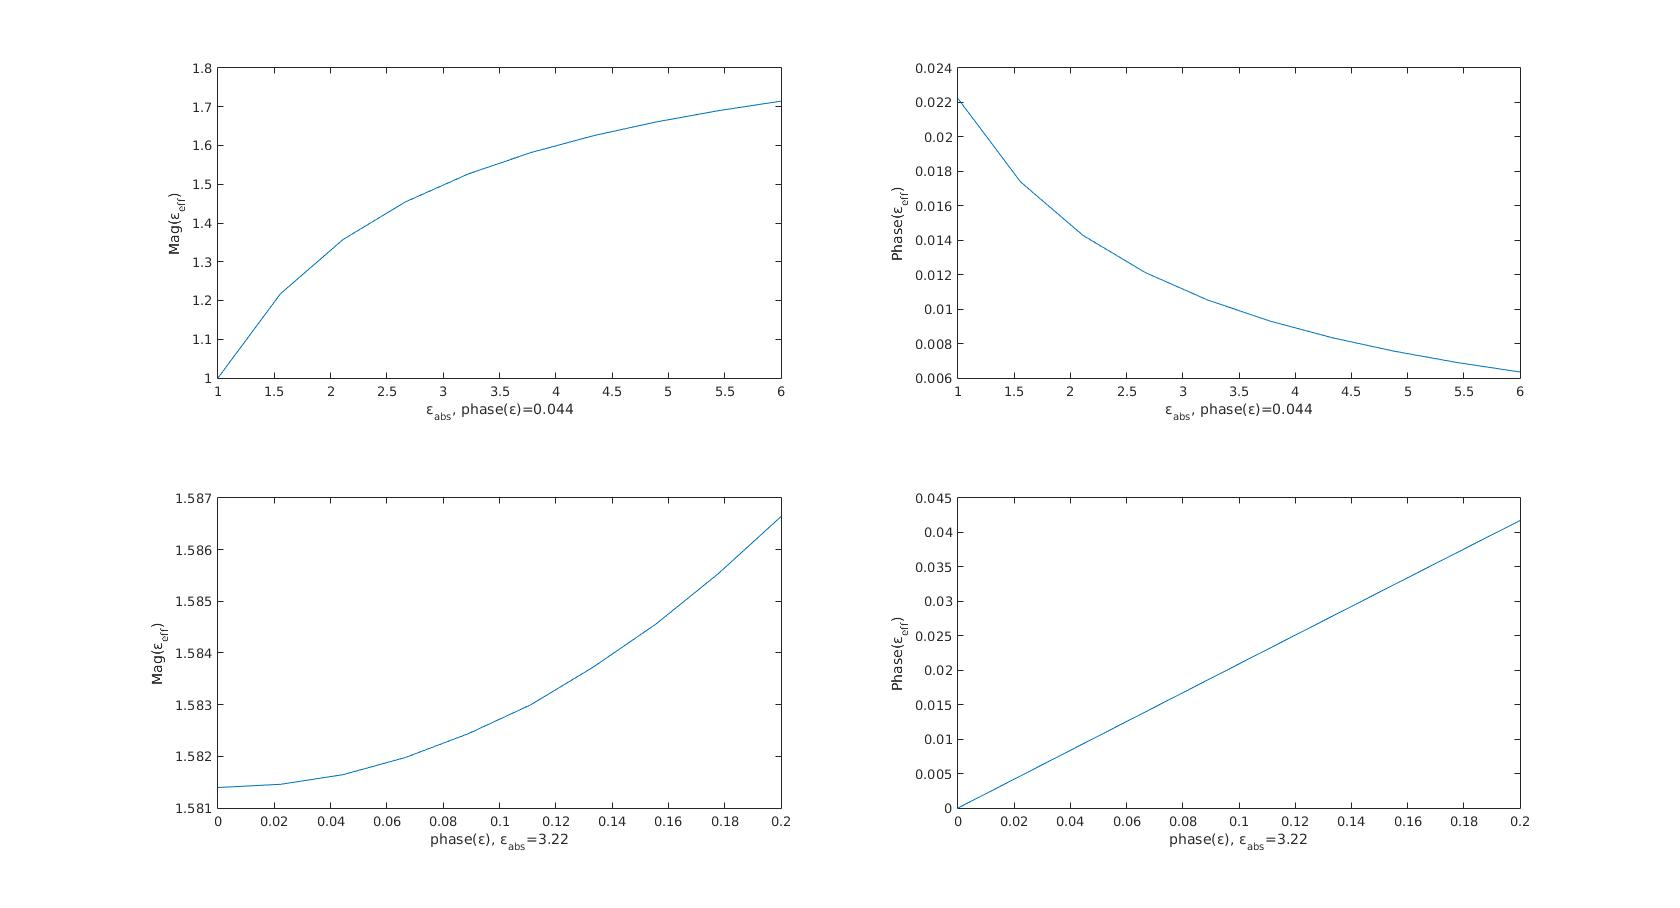
\includegraphics[width=\textwidth]{figures/Theory/layeredepsilon.jpg}
	
	\end{center}
	

\section{Clamping capability of Current Transformers }

\section{Noise Considerations}
\subsection{General}
The evaluation of noise added to the signal by the CT, the integrator, the BW-filter and the cables is of great importance as it limits the capability of measuring below-PD-currents though the capacitance of the specimen. 
In order to quantify the desired signal compared to the background noise, the Signal-to-Noise Ratio (SNF) can be measured. The SNF is a the ratio of signal power over signal noise. The power is proportional to the amplitude of the signal.
\begin{equation}
	SNF=P_{signal}/P_{noise} = (V_signal/V_noise)^2
\end{equation}
The degradation of the SNF is characterized by its input value over its output value, which is the Noise Figure (NF).
\begin{equation}
	NF = SNR_{in}/SNR{out}
\end{equation}
The amount of additional noise by the components can be characterized by the NF. 
\subsection{Noise of a Current Transformer}
A CT has an intrinsic noise that is caused by the Barkhausen noise of the magnetic core. It can be neglected as it is much lower than other sources of noise. %cite
Another noise source might occur due to the capacitive coupling of the primary wire to the copper case of the Current Transformer. This coupling capacitance might reach orders of a few picofarads. %\cite


\subsection{Noise of an Integrator}


